% This is a LaTeX template for a submission to American Journal of Political Science
% If you find any errors, please let me know: jjharden@unc.edu
\documentclass[12pt, letterpaper]{article}
 
%==============Packages & Commands=================
\usepackage{graphicx} % Graphics
\usepackage{epstopdf}
\usepackage{indentfirst} % Tells LaTeX to indent every paragraph 
\usepackage{setspace} % To set line spacing
\usepackage[longnamesfirst]{natbib} % For references
\usepackage{booktabs} % For tables
\usepackage{rotating} % For sideways tables/figures
\usepackage{amsmath} % Some math symbols
\usepackage[margin = 1in]{geometry}
\usepackage{subfig}
\usepackage{hyperref}
\usepackage{mdwlist}
\usepackage{url}
\usepackage{verbatim}
\usepackage{float}
\urlstyle{same}
\usepackage{multirow}
\newcommand{\R}{\texttt{R}\space} % Write R in typewriter font
\newcommand{\trans}[1]{{#1}^{\ensuremath{\mathsf{T}}}} % Transpose symbol 
\bibpunct{(}{)}{;}{a}{}{,} % Reference punctuation 
\captionsetup[subfloat]{position = top, font = large} % For sub-figure captions


%============Article Title, Authors================
\title{Forecasting Rebellion}
\author{John Beieler and Ben Fisher}

%===================Startup========================
\begin{document} 
\maketitle 

%================Begin Manuscript==================
\newpage
\doublespacing
\section*{Introduction}
Foreign policy is ultimately based on prediction. Policymakers base their decisions on how they think another state is going to react or respond. They are essentially making educated guesses based on the knowledge they have and the opinions of so-called area experts. In recent years, there has been a push to be more scientific in our predictions. The US government funds multiple projects, such as the Integrated Conflict Early Warning System (ICEWS) and the Political Instability Task Force (PITF), in an effort to develop statistical models capable of predicting events of interest. \\

\indent Unfortunately, the field of political science, particularly conflict studies, has lagged behind in this effort. Research pays more attention to finding statistically significant coefficient estimates using marginally different model specifications, rather than how well these models predict what they claim to explain. Our approach differs by focusing exclusively on developing models that are able to forecast. For the purposes of this study, we attempt to forecast the occurrence of rebellions in Southeast Asian countries using publicly available event data from the Global Database of Events, Language, and Tone (GDELT). We use several statistical methods from the field of data mining that we believe may be more useful than the linear regression methods commonly used in political science. \\

\indent Our paper proceeds as follows. First, we provide a brief overview of previous conflict-related forecasting research. A description of the data used follows and then a summary of the methods applied. Next, we discuss the results of our models. Finally, we conclude by providing an overview of our findings, as well as possible avenues for future research.\\

\section*{Review of Literature}
Conflict literature primarily tests hypotheses by looking for statistically significant coefficient estimates for key variables. The predictive ability of these models is rarely tested. Studies that have focused on testing the predictive ability of these models have proven that they are practically useless for forecasting their events of interest (King, Beck, & Zeng 2000; Ward, Greenhill, & Bakke 2010). As a result, there has being a growing call for the development of models with better forecasting ability (Schrodt 2013). Schrodt (2000) demonstrates that pattern recognition techniques used in conjunction with event data can be useful tools for predicting levels of conflict. The US government-backed ICEWS has had some success in predicting events of interest such as rebellions and domestic political crises in Southeast Asian countries using logistic regression in combination with event data and structural variables (O'Brien 2010). We previously expanded on the ICEWS approach by incorporating GDELT as a new source for the event data and models from data mining (Arva et al. 2013). This paper builds on the work in Arva et al. by narrowing the focus on optimizing our predictive accuracy using event data from GDELT. \\

\section*{Data}
Our data is derived from the GDELT dataset (http://gdelt.utdallas.edu), which is comprised of event data. At its core, event data records human interactions in a who-did-what- to-whom format using news stories as source material. For example, a news story that begins ``Syrian rebels attacked the town of Aleppo earlier Friday'' would be recorded as: source actor - SYRREB, target - SYR, event - 19. Using this underlying data, we construct a dataset that records counts of interactions between various groupings of actors. As an example, one such category records the number of violent events between government actors, such as a violent interaction between the governments of the United States and Russia. All told, our dataset has 70 columns recording these types of interactions for a group of countries involved in political events within Southeast Asia. For each country, time series of monthly data is constructed recording each of these counts. This data is fairly sparse, with a number of the 70 categories containing most, if not all, zeroes. The dependent variable in our analysis is whether a rebellion occurs within a given country within the next six months. This variable is dichotomous, and is coded a 1 if a rebellion occurred and 0 otherwise. This dependent variable is also rather sparse, with only 19\% of the data being coded as a positive observations. As an illustration of the data, for a country such as Cambodia, data on the interactions of Cambodian actors with other actors in January is recorded and used to predict whether a rebellion will happen within Cambodia in July. The total number of observations within the dataset is 4,350. \\

\section*{Method}

We perform tests using 4 different models: logistic regression, random forest, support vector machine, and adaptive 
boosting. We split the data into a 75-25\% train-test split before performing any analysis. Each start out with a 75-25\% 
split. All hyper-parameters are then tuned using 5-fold grid-search cross validation. Where appropriate (SVM) multiple 
rounds of k-fold CV are used to ensure unbiased estimates. The data is pre-divided in order to ensure that all the models 
are working with the same data so that estimates are consistent across models. The data is also scaled to have mean 0 and 
standard deviation of 1 for all models. This is especially important since our data is both sparse and has a wide range of 
values. \\

\section*{Experiments}

Following rounds of 5-fold cross validation, the following hyper-parameter settings are found to be optimal. For random 
forest, we use 250 trees, with trees grown to their maximum depth, the minimum number of samples for each split set to 1, 
and the Gini criterion used to determine splits. Adaptive boosting determines that the number of base estimators is 100, 
and we use the SAMME.R algorithm for the boosting portion. Logistic regression settles on a \texttt{C} parameter of 1, with 
class weightings inversely proportional to the class frequencies\footnote{This is the ``auto'' weighting in the scikit-learn Python library}, and L1 normalization. Finally, SVM settles on hyper-parameters of 2 for \texttt{C}, 
auto class weightings, an RBF kernel, and a gamma value of 0. The below table shows the results of various
metrics for these given models. \\

\begin{center} 
\begin{table}[H]
\caption{Model Scores}
\label{tab:results}
\centering
\begin{tabular}{l c c c} 
\hline\hline           
 Model              & Precision & Recall & F1  \\
\hline
AdaBoost            &  67\%           &  71\%           &  69\% \\
Logistic Regression &  63\%           &  \textbf{81\%}  &  71\% \\
Random Forest       &  \textbf{81\%}  &  74\%           &  \textbf{77\%} \\
SVM                 &  66\%           &  74\%           &  70\% \\
\hline
\multicolumn{3}{l}{Scores are from out-of-sample test set.} \\
\hline\hline
\end{tabular} 
\end{table}
\end{center}

We choose to present these scores rather than base accuracy scores due to the nature of our data: the data is unbalanced and we are attempting
to predict political behavior. This means that a raw accuracy score is not the best descriptor of model performance for our situation. 
Given this, we use the precision, recall, and F1 scores, with the precision score representing how well a classifier 
can avoid labeling a negative sample as positive, recall representing how well all the positive observations can be found, and the F1 score the 
weighted combination of the two. The above table shows that the random forest performs best on both precision and F1 scores, while the logistic
regression is best at picking out the positive observations. In addition, we present ROC curves and classification tables in order to better
understand our results.\\

\begin{center}
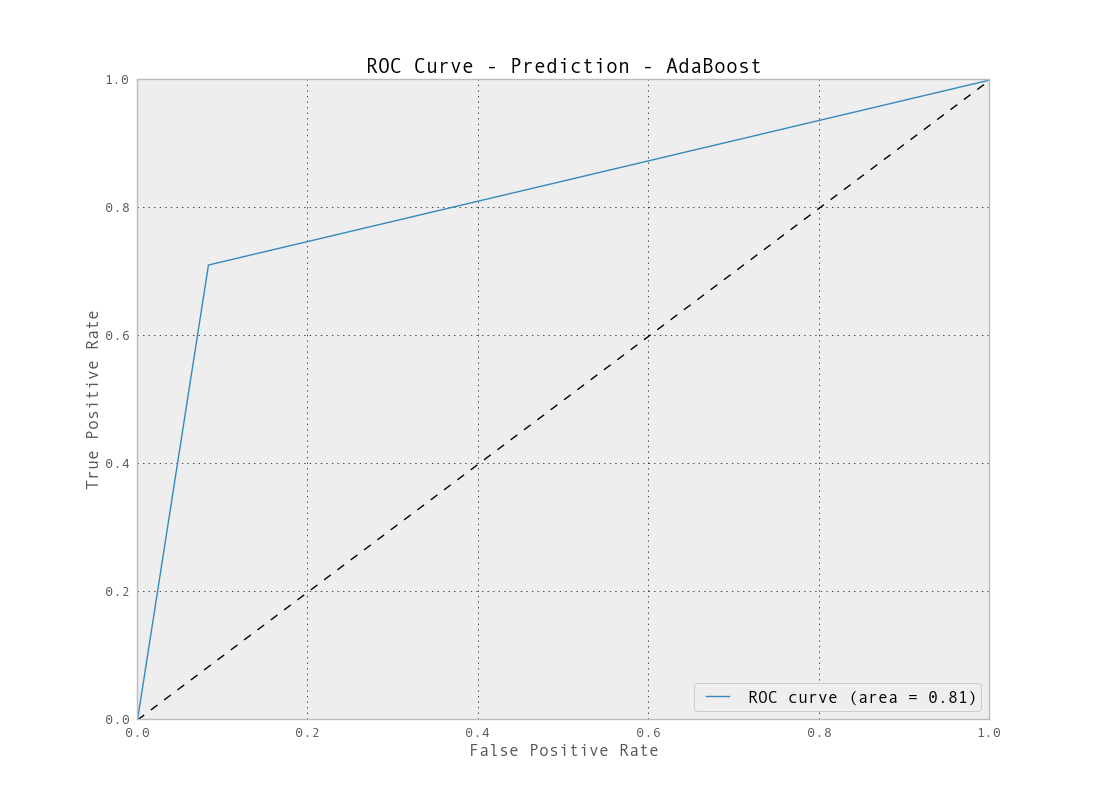
\includegraphics[height=5in, width=5in]{roc_plot_Prediction_AdaBoost.png}
\end{center}

\begin{center}
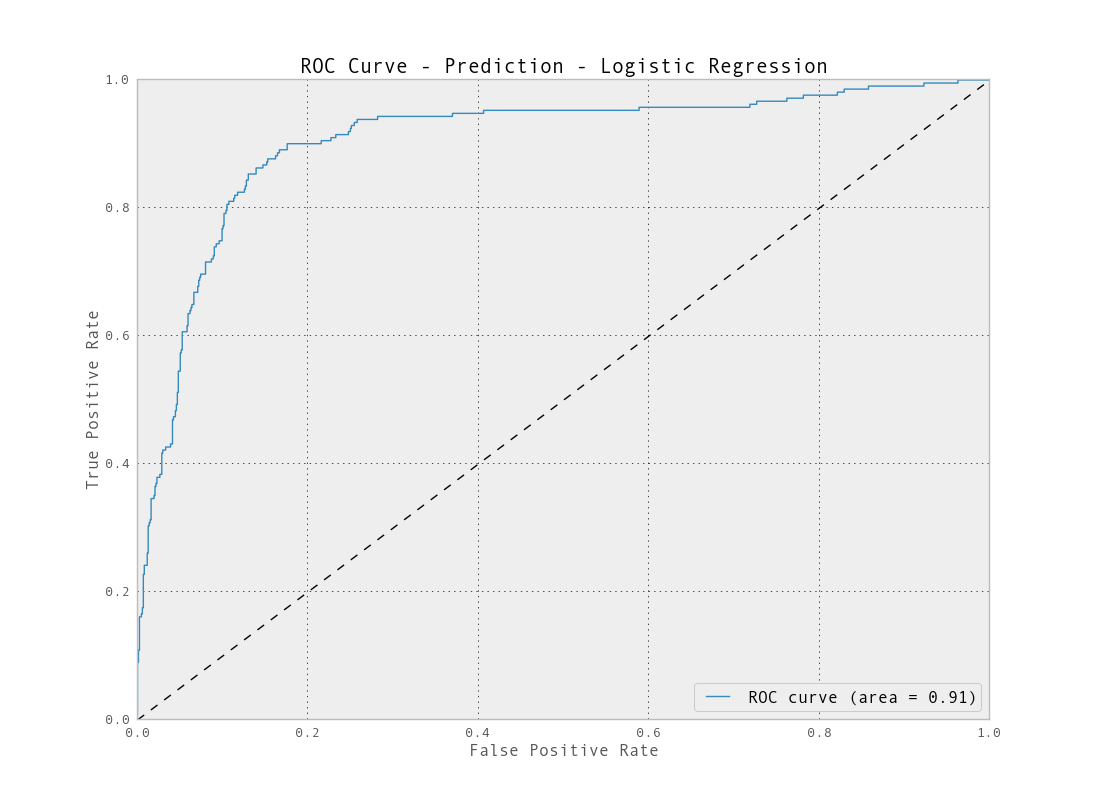
\includegraphics[height=5in, width=5in]{roc_plot_Prediction_LogisticRegression.png}
\end{center}

\begin{center}
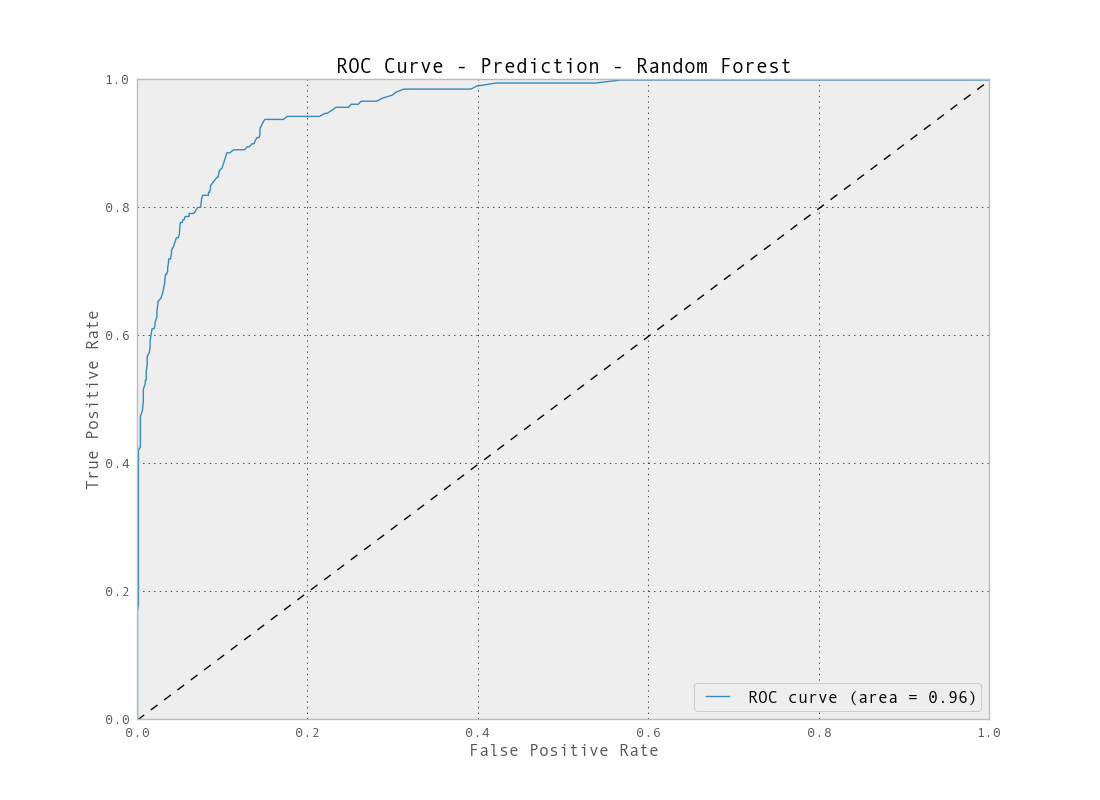
\includegraphics[height=5in, width=5in]{roc_plot_Prediction_RandomForest.png}
\end{center}

\begin{center}
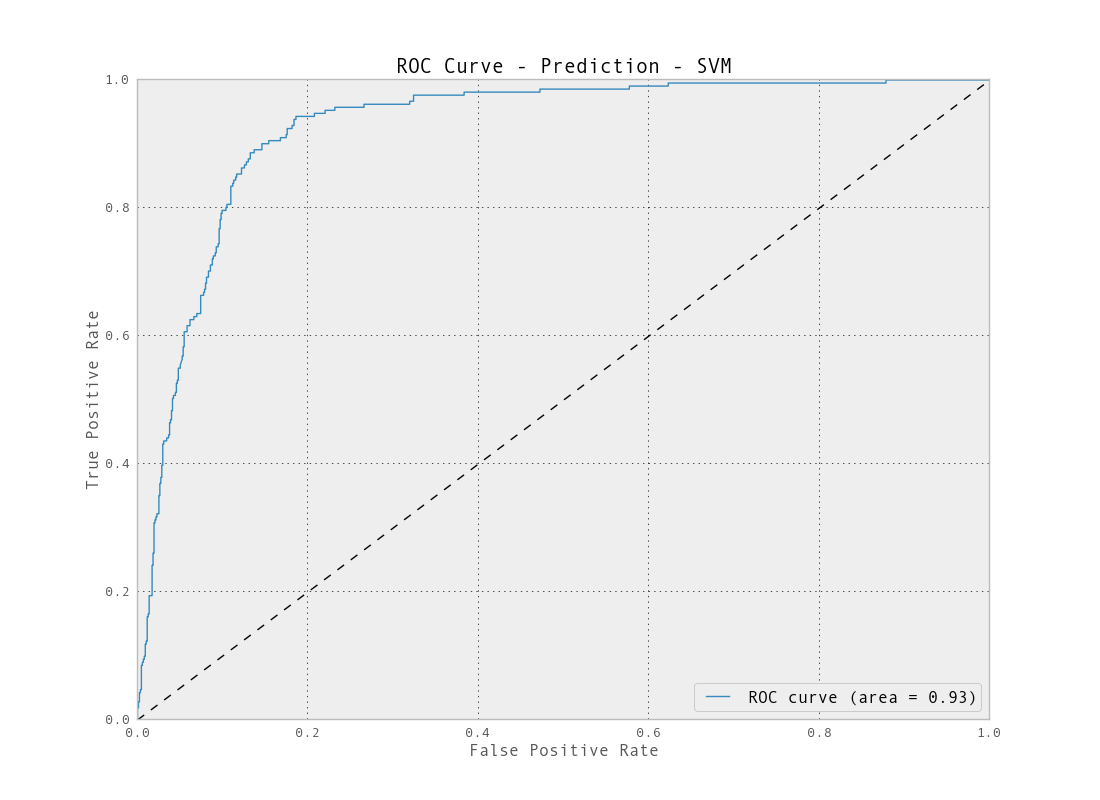
\includegraphics[height=5in, width=5in]{roc_plot_Prediction_SVM.png}
\end{center}

\begin{center} 
\begin{table}[H]
\caption{Classification Table - AdaBoost}
\label{tab:6domcri}
\centering
\begin{tabular}{c c c} 
\hline\hline           
 & \multicolumn{2}{c}{Predicted} \\
 Actual & 0 & 1 \\
 \hline
 0  & 804 & 73 \\
 \\
 1  & 61 & 150 \\
\hline
\end{tabular} 
\end{table}
\end{center}

\begin{center} 
\begin{table}[H]
\caption{Classification Table - Logistic Regression}
\label{tab:6domcri}
\centering
\begin{tabular}{c c c} 
\hline\hline           
 & \multicolumn{2}{c}{Predicted} \\
 Actual & 0 & 1 \\
 \hline
 0  & 778 & 99 \\
 \\
 1  & 40 & 171 \\
\hline
\end{tabular} 
\end{table}
\end{center}

\begin{center} 
\begin{table}[H]
\caption{Classification Table - Random Forest}
\label{tab:6domcri}
\centering
\begin{tabular}{c c c} 
\hline\hline           
 & \multicolumn{2}{c}{Predicted} \\
 Actual & 0 & 1 \\
 \hline
 0  & 840 & 37 \\
 \\
 1  & 55 & 156 \\
\hline
\end{tabular} 
\end{table}
\end{center}

\begin{center} 
\begin{table}[H]
\caption{Classification Table - SVM}
\label{tab:6domcri}
\centering
\begin{tabular}{c c c} 
\hline\hline           
 & \multicolumn{2}{c}{Predicted} \\
 Actual & 0 & 1 \\
 \hline
 0  & 796 & 81 \\
 \\
 1  & 55 & 156 \\
\hline
\end{tabular} 
\end{table}
\end{center}

%Analysis of the results. Random forest will likely win. Nonparametric. Doesn't care about functional form. Yadda yadda.

In general, it appears that the random forest performs the best. This is to be expected for a few reasons. First, the fact that random forest is 
nonparametric and ignores the functional form of the data should make it better suited to our analysis than parametric models. This is important 
since our data is highly complicated, even post scaling. Additionally, the random forest is able to construct complex decision rules that
fully capture the nature of the underlying processes that lead our outcome of interest, rebellions.\\

All of the models seem to achieve good accuracy. SVM performs the best with a mean accuracy of about 93\%. However, the other models are not far 
behind. Random forest has an accuracy of just over 91\%, while logistic regression and adaptive boosting each achieve approximately 89\% accuracy. 
Random forest has the best precision, F1 score, and the most area under the curve (AUC), while logistic regression has the best recall. Adaptive 
boosting is clearly at the bottom in terms of performance.\\

Highest accuracy is not necessarily an indicator of the best model in our case. Because our dependent variable is relatively sparse, one could 
achieve 81\% accuracy by simply predicting that there will never be any rebellions. This does us no good. We are ultimately concerned with 
identifying when a rebellion will occur so that policymakers can react accordingly. Because one of the aims of our research is to be policy 
relevant, we are more interested in minimizing false negatives, rather than false positives. It is a "better safe than sorry" approach. We would 
prefer that policymakers prepare for a rebellion that does not occur instead of predicting no rebellion and being caught by surprise.\\ 

With this in mind, it becomes a decision between between logistic regression and random forest. While random forest has a better overall accuracy, 
it has more false negatives and fewer true positives than logistic regression. Logistic regression does a superior job of minimizing the false 
negatives. However, it generates many more false positives than random forest. In this case, logistic regression is probably better suited to our 
analysis due to our goal of minimizing false negatives. \\

In terms of features, the one that consistently appears most often as an ``important'' feature is \texttt{gov\_opp\_matcf}.
This represents the number of physically conflictual, e.g., an attack, events between government actors and opposition
actors. For example, if the Syrian government attacks a Syrian opposition group, this would count as a 
\texttt{gov\_opp\_matcf} event. Intuitively, it makes sense why this variable will be important for predicting whether a 
rebellion will occur; the more violent the government is towards the groups that oppose it, the more likely there is to
be a rebellion by those opposition groups. Other important variables capture the interactions between government actors, 
e.g., actions between the Syrian government and the U.S. government. This finding is also unsurprising, since the actions
of one government may serve to temper or exacerbate the actions of another.\\

%Novel ideas. Data is unbalanced. We can implement reweighting of the results by doubling up the positive observations to deal with false negatives. We could try mulitiplicative or polynomial features, but we're getting pretty good results as it is.

There are a few ways we could potentially improve our accuracy. The main issue we have is that our data is unbalanced, with many more 0s than 1s. 
We could correct for this by reweighing the observations and doubling the number of positive observations. This could help achieve our goal of 
reducing false negatives. We could also transform our features using multiplicative or polynomial terms. Finally, we might see improvement if we 
also included non-event variables, such as GDP, ethnic fractionaliztion, etc., into our models. This would likely give a better idea of which 
states are more susceptible to rebellion generally than others. Of course, all this is not to say we are unhappy with our results. Our mean 
accuracy is very high, as well as the scores for the other metrics. The fact that we are achieving these kind of results in our first attempt is 
very promising.\\

\section*{Future Work}

%Doesn't take into account autoregressive properties. There are lots of other features in GDELT that we don't take into account (e.g., geolocations).

There is still much work to be done. Right now, we do not use all the data we probably should. We are currently making predictions using data six 
months prior to our month of interest and ignoring all months before that. Future work should find a way to incorporate and weight data from the 
months leading up to the six month cutoff. \\

In addition, we may not be predicting our real event of interest in our data's current form. Our primary goal is really to predict the onset of 
rebellion, and we do not know for sure if the analysis in this paper actually does that. The dependent variable is coded as 1 for all months when a 
rebellion is active. A better approach would be to code only the month when a rebellion begins and when a rebellion ends. We could then alter the 
independent variables from counts to the change in the number of events from the previous month to better capture the change from peace to conflict 
and conflict to peace. \\

As previously discussed, future research should also include non-event variables. While this covers commonly used structural variables, we are most 
interested in making better use of the GDELT data. We are particularly interested in incorporating its geolocation data into future models.
This should allow us to better pinpoint where we expect conflict to occur within a country and allow us to understand how it spreads.\\

%Expensive to obtain labels of data? Noises and uncertainties in the data? How can we consider human factor in the mining process? How can we bridge the gap between discovered patterns and decision making?  

%All of the above. Coding of the DV requires human intervention. GDELT is extremely messy and has varying levels of coverage. IDK about human factors. Bridge the gap...we can riff off of story telling here if we need to fill in space. 

Conflict forecasting research faces several challenges. First of all, data availability limits us. While the GDELT data are updated on a daily basis, we have to either rely on human-coded data for our dependent variable or code it ourselves. This also means that our event of interest is sensitive to how the coders define it. Determining when exactly a rebellion began may be a matter of opinion, and whether the occurrence of internal conflict even constitutes a rebellion is another issue. The GDELT data presents other sorts of problems. The data is very noisy and unbalanced. As a result, we have to develop methods of correcting for this in our analyses. \\

This paper contributes to the field of conflict forecasting by testing the utility of several models from data mining using event data from the recently released GDELT dataset. Overall, we achieve very good results, with logistic regression performing the best for our purposes. Future research should focus on predicting rebellion onset specifically and include structural and geographical data. While it is unlikely that there will ever be a philosopher's stone of conflict forecasting, a model that turns common events into perfect predictions, the field is making great strides in terms of predictive ability and policy relevance.

\section*{References}
\noindent Arva, Bryan, Ben Fisher, Gustavo Lara, Philip A. Schrodt, Wonjun Song, Marsha Sowell\\ 
\indent and Sam Stehle. "Improving Forecasts of International Events of Interest." Annual 
\indent Meeting of the European Political Studies Association. Barcelona. June 2013.\\
Beck, Nathaniel, Gary King, and Langche Zeng. "Improving Quantitative Studies of\\ 
\indent International Conflict: A Conjecture." \emph{American Political Science Review} 94 (2000),\\ \indent 21-35.\\
\noindent OÕBrien, Sean P. 2010. ÒCrisis early warning and decision support: Contemporary approaches 
\indent and thoughts on future research.Ó International Studies Review 12(1):87Ð104.\\
\noindent Schrodt, Philip A. "Pattern recognition of international crises using hidden Markov models." 
\indent Political complexity: Nonlinear models of politics (2000): 296-328.\\
\noindent Schrodt, Philip A. ``Seven deadly sins of contemporary quantitative political analysis." 
\indent Proc. APSA 2010 (2010).\\
\noindent Ward, Michael D., Brian D. Greenhill, and Kristin M. Bakke. "The perils of policy by p-
\indent value: Predicting civil conflicts." Journal of Peace Research 47.4 (2010): 363-375.\\
\end{document}